% 三角恒等式

\pentry{三角函数}

这里列出几个高中常见的三角函数恒等式, 推导从略. 以下用到的两个高中不常见的三角函数分别为 $\csc x= 1/\sin x$, $\sec x = 1/\cos x$, 分别读作 cosecant 和 secant\\

\noindent\bb{勾股定理}

\begin{equation}
\sin^2 x + \cos^2 x = 1
\end{equation}
等式两边同除 $\cos^2 x$ 得
\begin{equation}\label{TriEqv_eq13}
\tan^2 x + 1 = \sec^2 x
\end{equation}

\noindent\bb{两角和公式}
\begin{gather}\label{TriEqv_eq1}
\sin(x\pm y) = \sin x\cos y \pm \cos x\sin y\\
\cos(x\pm y) = \cos x\cos y \mp \sin x\sin y
\end{gather}

\noindent\bb{二倍角公式}

令\autoref{TriEqv_eq1} 中 $y=x$ 取上号得
\begin{gather}
\sin 2x = 2\sin x\cos x\\
 \cos 2x = \cos^2 x - \sin^2 x \label{TriEqv_eq4}
\end{gather}

\noindent\bb{降幂公式}

结合\autoref{TriEqv_eq4} 和 $\sin^2 x + \cos^2 x = 1$ 可以得到
\begin{gather}
\sin^2 x = \frac12 (1- \cos 2x) \label{TriEqv_eq5} \\
\cos^2 x = \frac12 (1+\cos 2x) \label{TriEqv_eq6}
\end{gather}

\noindent\bb{和差化积公式}
\begin{gather}
\sin x + \sin y = 2\sin\qty(\frac{x + y}{2})\cos\qty(\frac{x - y}{2})\label{TriEqv_eq7}\\
\sin x - \sin y = 2\sin\qty(\frac{x - y}{2})\cos\qty(\frac{x + y}{2})\label{TriEqv_eq8}\\
\cos x + \cos y = 2\cos\qty(\frac{x+y}{2})\cos\qty(\frac{x-y}{2})\label{TriEqv_eq9}\\
\cos x - \cos y = -2\sin\qty(\frac{x+y}{2})\sin\qty(\frac{x-y}{2})\label{TriEqv_eq10}
\end{gather}

这里介绍一种推导方法可方便记忆. 以\autoref{TriEqv_eq9} 为例, $\cos x, \cos y$ 和 $\cos x + \cos y$ 分别等于\autoref{TriEqv_fig1} 中矢量 $\vec A, \vec B$ 和 $\vec A + \vec B$ 在水平方向的投影长度, 而 $\vec A + \vec B$ 在水平方向的投影长度等为 $\abs{\vec A + \vec B}\cos[(x+y)/2]$, 其中 $\abs{\vec A + \vec B} = 2\cos [(y-x)/2]$, 代入可得\autoref{TriEqv_eq9}. 利用 $\vec A + \vec B$ 在竖直方向的投影可得\autoref{TriEqv_eq7}, 把\autoref{TriEqv_eq7} 和\autoref{TriEqv_eq9} 中的 $y$ 分别替换成 $-y$ 和 $y+\pi$ 可推导出\autoref{TriEqv_eq8} 和\autoref{TriEqv_eq10}.
\begin{figure}[ht]
\centering
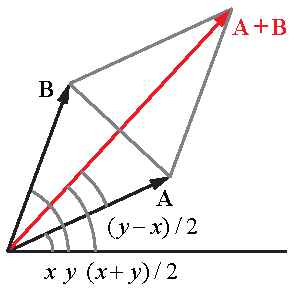
\includegraphics[width=5.5cm]{./figures/TriEqv1.pdf}
\caption{和差化积公式推导} \label{TriEqv_fig1}
\end{figure}